\chapter{Nulla-ismeretű protokoll}

A nulla-ismeretű protokollok a kihívás-válasz protokollokkal szemben képesek úgy bizonyítani a titok ismeretét, hogy nem adnak semmilyen információt a róla. Hogy lássuk hogyan is működik, a formális definíció előtt egy egyszerű példával szeretném szemléltetni \cite{ZKPToYourChildren, schneier2015applied}.

A \ref{Figure::ZKcave} ábrán látható egy barlang. A \textit{C} és \textit{D} pontok között található egy ajtó, amely egy jelszóval nyílik. Ehhez az ajtóhoz csak Aladár tudja a jelszót, senki más. Aladár be szeretné bizonyítani Krisztának, hogy tudja a jelszót, de ezt a jelszó megosztása nélkül szeretné megtenni. A következő a menete Aladár bizonyításának.

\begin{enumerate}
    \item Kriszta megáll az \textit{A} pontnál.
    \item Aladár elsétál a barlangban egészen a \textit{C} vagy \textit{D} pontig.
    \item Ezt követően Kriszta elsétál a \textit{B} pontig, így ő nem tudja, hogy Aladár melyik irányba ment.
    \item Kriszta kiált Aladárnak, hogy:
        \begin{itemize}
            \item a bal útvonalról érkezzen.
            \item a jobb útvonalról érkezzen.
        \end{itemize}
    \item Aladár kinyitja az ajtót, ha szükséges és a kívánt irányból érkezik Krisztához.
    \item Aladár és Kriszta annyiszor ismétlik a lépéseket az 1. lépéstől az 2. lépésig ahányszor szükséges a bizonyításhoz.
\end{enumerate}

\begin{figure}[H]
    \centering
    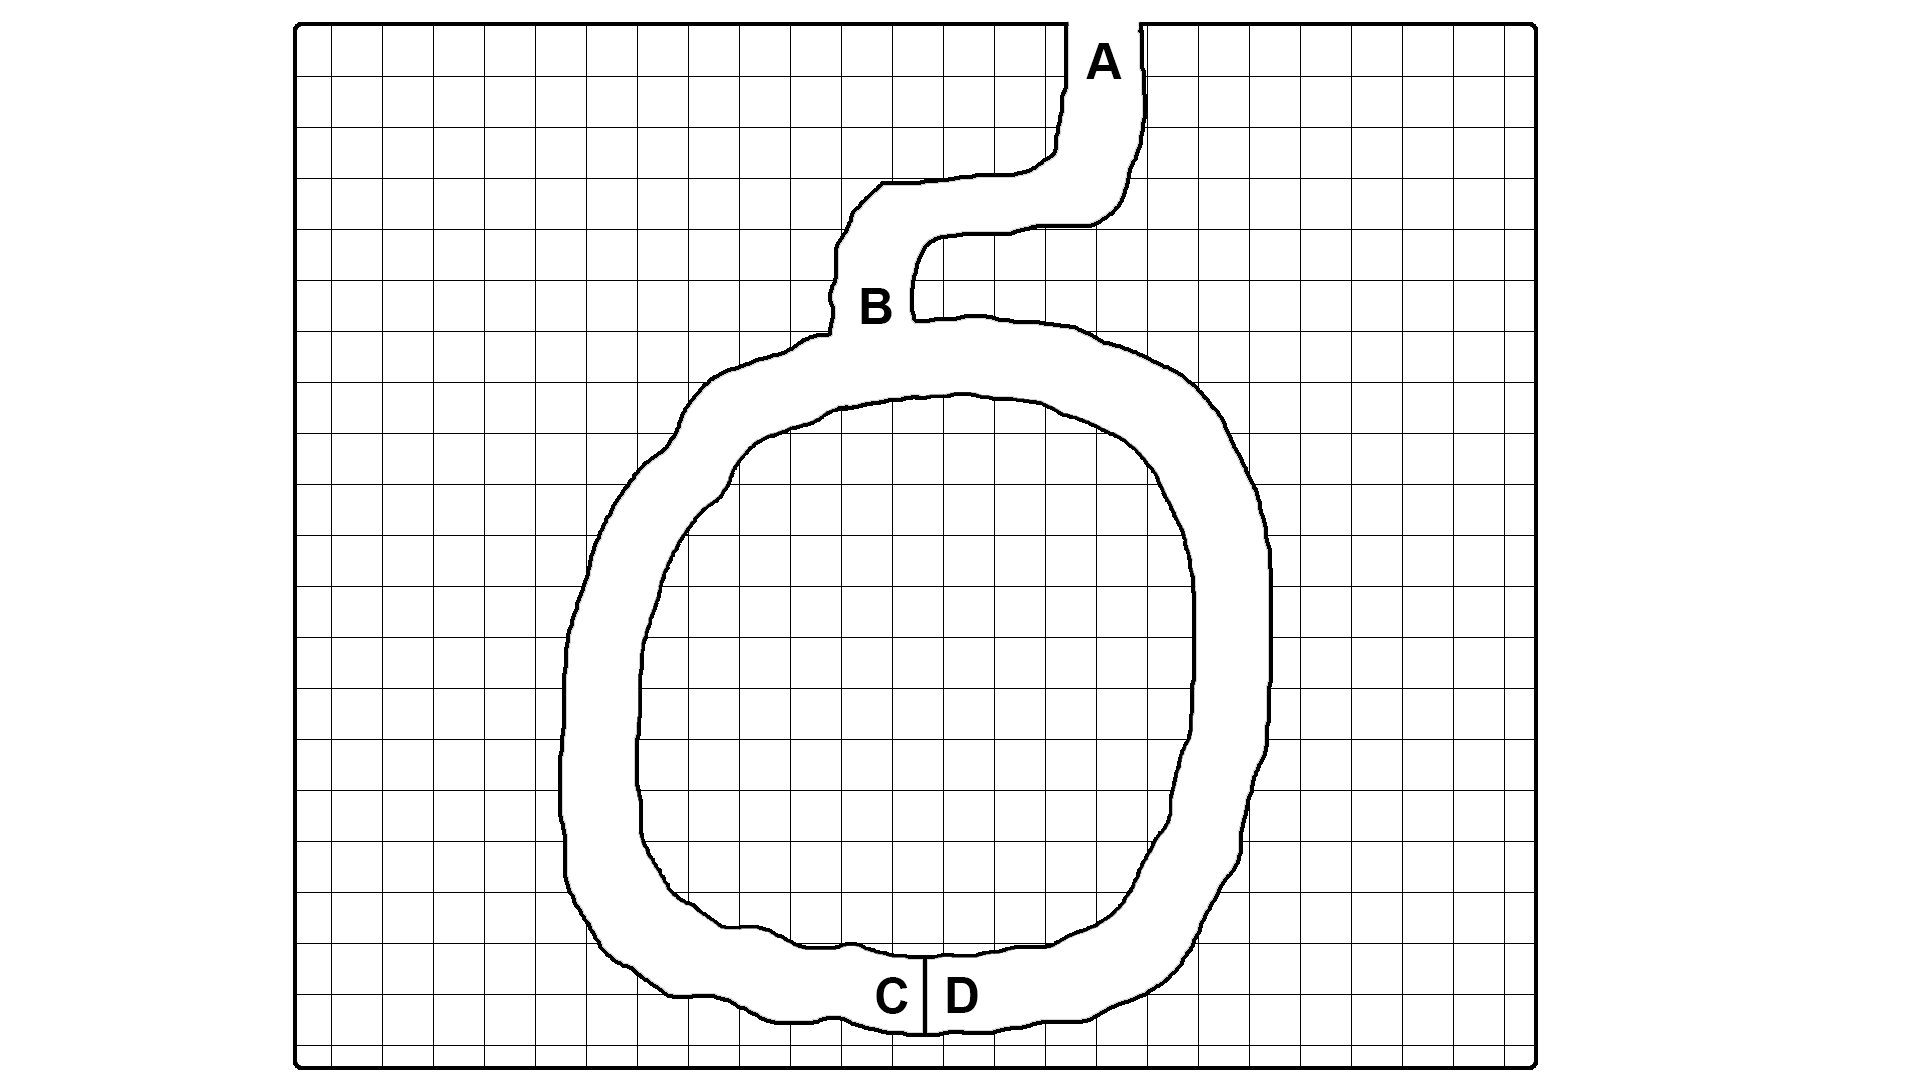
\includegraphics[width=0.6\textwidth]{ZKP.png}
    \caption{A nulla-ismeretű barlang.}
    \label{Figure::ZKcave}
\end{figure}

A többszöri ismétlésre azért van szükség, mert lehet Aladár be szeretné csapni Krisztát, amire minden iterációban 50\% esélye van. Ha abba az irányba ment amelyet Kriszta kiált, akkor szerencsésen be tudta őt csapni, azonban megfelelő ismétlésszámmal sokkal kevesebb esélye van Aladárnak.

A példa egy másik fontos jellemzője az, hogy Aladár ezzel bebizonyíthatta Krisztának, hogy tudja a jelszót, azonban Kriszta nem tud meggyőzni más arról, hogy Aladár tudja a jelszót. Tegyük fel, hogy Kriszta videót készített az egész folyamatról, de így se képes ő maga bizonyítani, hiszen mondhatjuk, hogy a felvétel hamisított, csalás.

Belátható, hogy ez egy nulla ismeretű protokoll, hiszen Kriszta számára bebizonyította Aladár, hogy ismeri a jelszót, méghozzá úgy hogy Kriszta semmit se tudott meg a jelszóról. Emellett Kriszta nem képes bizonyítani harmadik fél számára, hogy Aladár tudja a jelszót.

A nulla-ismeretű protokollokat Menezes, Oorschot és Vanstone a következő módon írták le formálisan könyvükben \citeyear{menezes1997handbook}:

Tekintsünk a nulla-ismeretű protokollokra kezdetben, mint interaktív bizonyítási rendszerekre (intaractive proof system), amiben a bizonyító és a hitelesítő felek többször is üzenetet váltanak. A bizonyjtó célja az, hogy valamilyen módon meggyőzze az hitelesítő felet, hogy birtokában van valamilyen tudásnak. A hitelesítő pedig elfogadhatja vagy elutasíthatja a bizonyítékot. A több üzenetváltásra azért van szükség, mert a bizonyíték egy interaktív játék formájában jön létre, ami egy inkább valószínűségi bizonyíték, mint abszolút bizonyíték. A hitelesítőn múlik, hogy milyen bizonyossággal rendelkező bizonyítékot fogad el, ez általában egy 1-hez rendkívül közeli érték szokott lenni.

Egy interaktív bizonyítékra azt mondjuk, hogy a \textit{proof of knowledge}, ha rendelkezik a \textit{teljesség} (completeness) és \textit{megalapozottság} (soundness) tulajdonságokkal.

\begin{definition}
    \textbf{Teljesség.} Egy interaktív bizonyíték teljes, ha adott egy becsületes bizonyító és egy becsületes hitelesítő, valamint a protokoll sikeresen megy végbe (a hitelesítő elfogadja a bizonyító állítását).
\end{definition}

\begin{definition}
    \textbf{Megalapozottság.} Egy interaktív bizonyíték \textit{megalapozatlan}, ha létezik egy polinomiális algorimtus \textit{M} a következő tulajdonsággal: ha egy tisztességtelen bizonyító (megszemélyesíti Aladárt) nem elhanyogalható valószínűséggel sikeresen tudja végrehajtani a protokollt a hitelesítő féllel (Krisztával), akkor \textit{M} segítségével kinyerhető a a valódi bizonyító (Aladár) tudása/titka, amely így felhasználható a későbbiekben a protokoll futtatásakor.
\end{definition}

Mivel minden olyan félnek, aki képes Aladárt megszemélyesíteni, valójában a titokkal egyenértékű ismerettel kell rendelkeznie, a \textit{megalapozottság} tulajdonság garantálja, hogy a protokoll valóban előállítja a \textit{tudás bizonyítékát}. Így ez a tulajdonság megakadályozza a csalókat.

Míg a fenti tulajdonságok lefekteti a nulla-ismeretű protokollok alapját, a legfőbb tulajdonság, amiről a nevüket is kapták, a \textit{nulla-ismeret}.

Azonban mielőtt kitérnénk erre a definícióra, szükséges megismernünk mik is a \textit{szimulátorok}. A barlangos példa esetében előjött egy eset, hogy Kriszta felvételt készít Aladár bizonyításáról és beláttuk hiába mutatja azt meg egy harmadik félnek, ő nem fogja elhinni, mert nem megbízható a felvétel mint bizonyíték (könnyen hamisítható). A harmadik fél csak úgy lenne meggyőzhető, ha Aladár eljátszaná a bizonyítást a harmadik fél által választott szekvenciára. Ha létezik olyan módszer, amellyel készíthető az eredetitől megkülönböztethetetlen bizonyíték, akkor azt mondjuk hogy létezik \textit{szimulátor} a bizonyítékra.

\begin{definition}
    \textbf{Nulla-ismeret.} Egy \textit{proof of knowledge} protokoll, rendelkezik a nulla-ismeret tulajdonsággal, ha szimuláltható a következő módon: létezik egy polinomiális algoritmus (\textit{szimulátor}), amely a valódi bizonyító féllel való együttműködés nélkül képes az bemenetnek megfelelő átiratot készíteni, amely megkülönböztethetetlen a valódi bizonyító féltől kapottól.
\end{definition}

A \textit{nulla-ismeret}-ből következik, hogy ha a bizonyító fél végrehajtja a protokollt, azzal nem ad ki semmilyen információt a titokról, csupán bizonyítja a tudását. Így akárhányszor is bizonyítja, a megszemélyesítése nem lesz egyszerűbb.